%% example.tex
%% Jeremy Singer
%% 16 Oct 12

\documentclass{mpaper}

\begin{document}

\title{An Example Paper for MSci Submission}
\author{Jeremy Singer}
\matricnum{12345678}

\maketitle

\begin{abstract}
According to Simon Peyton Jones, an abstract should address
four key questions. First, what is the problem that this
paper tackles? Second, why is this an interesting problem?
Third, what is the solution this paper proposes?
Finally, why is the proposed solution a good one?
\end{abstract}

\section{Introduction}

This paper outlines the standard template for an MSci submission.
In earlier years, MSci students at the School of Computing
Science\footnote{\url{http://www.dcs.gla.ac.uk}},
University of Glasgow, were expected to produce a full-length
dissertation. Now, the requirement is for MSci students to
write a paper of up to 14 pages in length, using the supplied
\texttt{mpaper} \LaTeX style file.

The precise structure of an MSci paper is not mandated, but it should
probably cover in detail the following aspects of the project.
\begin{enumerate}
\item General description of the problem, motivation, relevance
\item Background information, possibly including a literature survey
\item Description of approach taken to solve the problem, including
  high-level design and lower-level implementation details as appropriate
\item Evaluation, qualitative or quantitative as appropriate
\item Conclusion, including scope for future work
\end{enumerate}

\section{Background}

This \LaTeX template is based on the ACM \texttt{sig-alternate} class.
The layout is two-column text. Generally figures and tables only
extend to one column width, e.g.\ Table \ref{tab-eg},
but it is possible to make them
stretch over both columns using the \texttt{figure*} and
\texttt{table*} environments. For an example, see Figure \ref{fig-eg}.

\begin{table}
\begin{tabular}{l||c||p{2cm}}
\emph{Operating System} & \emph{Version} & \emph{Verdict} \\ \hline \hline
Ubuntu & 12.04 & Everyone's favourite Linux, unless you grew up with
RedHat \\ \hline
Slackware & xxx & Pseudo-hacker's Linux, how often do you recompile
your kernel? \\ \hline
Mac OS & 10.7 & For people with more money than sense \\ \hline
\end{tabular}
\caption{\label{tab-eg}Single column table of figures}
\end{table}

\begin{figure*}
\begin{center}
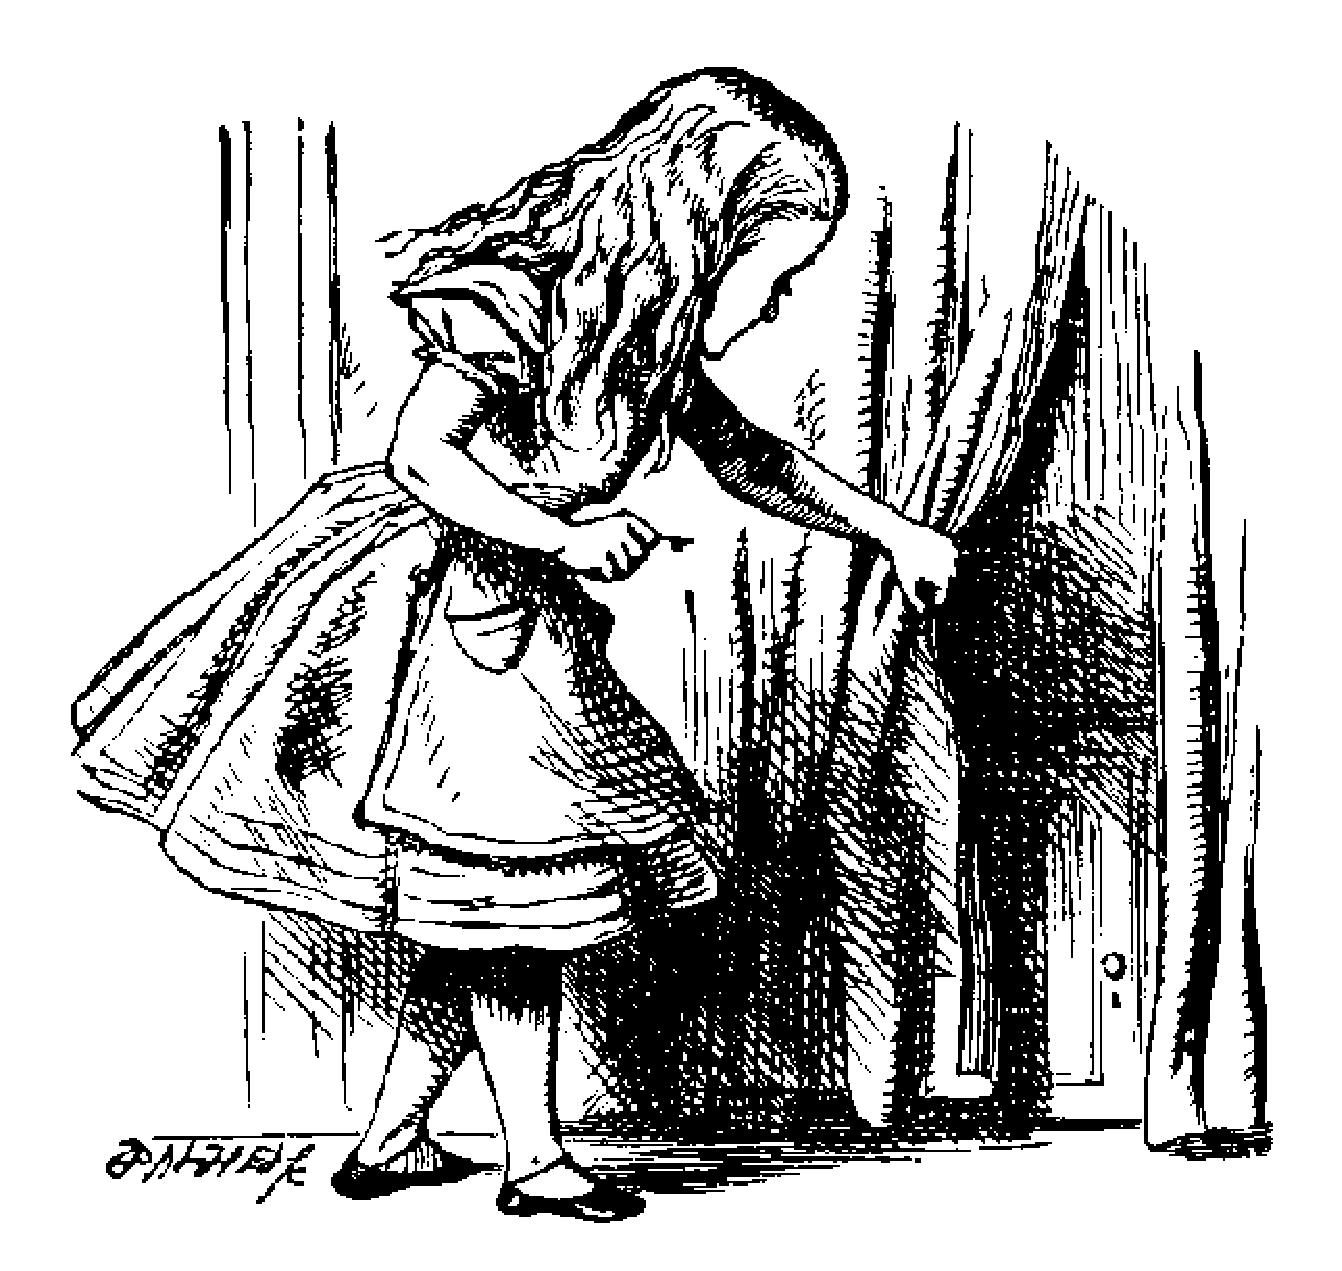
\includegraphics[scale=0.3]{alice.pdf}
\end{center}
\caption{\label{fig-eg}An example figure stretching over two columns}
\end{figure*}

\section{The WizWoz System}

Again, Simon Peyton Jones has a lovely description of how to write a
paper on his
website\footnote{\url{http://research.microsoft.com/en-us/um/people/simonpj/papers/giving-a-talk/giving-a-talk.htm}}.
Personally, I put URLs in footnotes and \emph{bona fide} references
in the bibliography. For instance, Turing \cite{turing37computable}
and Knuth \cite{knuth68art} would not be out of place in list of
references.
How many references? Hard to say. Five is not enough, 50 is pushing
it.

\subsection{User Interface}

Blah blah blah
Blah blah blah
Blah blah blah
Blah blah blah

% - - - - - - - - - - - - - - - - - - - - - - - - - - - - - - - - - - - - - - -
\subsection{Foo}

Blah blah blah
Blah blah blah
Blah blah blah

\subsubsection{Bar}
\textsf{Blah} \textit{blah} \textbf{blah}

\section{Evaluation}

Graphs are always good. I recommend getting to grips with Matlab, R or
gnuplot rather than exporting horribly Excel bitmapped graphs.


\begin{quotation}
 The Assyrian came down like the wolf on the fold,
 And his cohorts were gleaming in purple and gold;
 And the sheen of their spears was like stars on the sea,
 When the blue wave rolls nightly on deep Galilee.

 Like the leaves of the forest when Summer is green,
 That host with their banners at sunset were seen:
 Like the leaves of the forest when Autumn hath blown,
 That host on the morrow lay withered and strown.
\end{quotation}

\section{Conclusions}

The standard Lorem Ipsum passage, used since the 1500s

``Lorem ipsum dolor sit amet, consectetur adipisicing elit, sed do eiusmod tempor incididunt ut labore et dolore magna aliqua. Ut enim ad minim veniam, quis nostrud exercitation ullamco laboris nisi ut aliquip ex ea commodo consequat. Duis aute irure dolor in reprehenderit in voluptate velit esse cillum dolore eu fugiat nulla pariatur. Excepteur sint occaecat cupidatat non proident, sunt in culpa qui officia deserunt mollit anim id est laborum.''
\vskip8pt \noindent
{\bf Acknowledgments.}
This is optional; it is a location for you to thank people

\bibliographystyle{abbrv}
\bibliography{example}


\end{document}